\def\dlt{0.4}
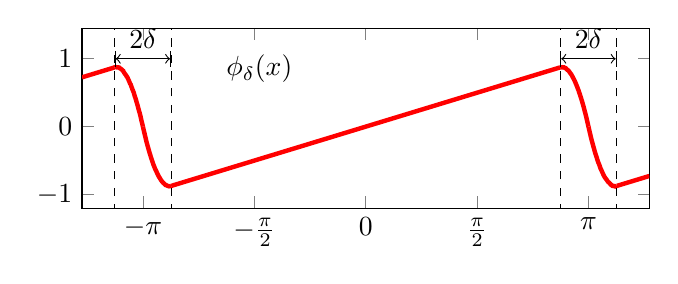
\begin{tikzpicture}
\begin{axis}[
    width=250pt,height=110pt,
    xmin=-4,xmax=4,
    ymin=-1.2,ymax=1.45,
    samples=50,
    xtick={-pi, -pi/2, 0, pi/2, pi},
    xticklabels={$-\pi$, $-\frac{\pi}{2}$, $0$, $\frac{\pi}{2}$, $\pi$},
    grid style={line width=.1pt, draw=gray!10}]
    
    \addplot[red, ultra thick, domain=-pi+\dlt:pi-\dlt] (x, x/pi);
    \addplot[red, ultra thick, domain=-4:-pi-\dlt] (x, x/pi + 2);
    \addplot[red, ultra thick, domain=pi+\dlt:4] (x, x/pi - 2);

    \addplot[red, ultra thick, domain=-pi:-pi+\dlt] (x, x/pi + x*x/\dlt/\dlt + 2*pi*x/\dlt/\dlt - 2*x/\dlt + 1 + pi*pi/\dlt/\dlt - 2*pi/\dlt);
    \addplot[red, ultra thick, domain=-pi-\dlt:-pi] (x, 1 - 2*pi/\dlt - 2*x/\dlt + x/pi - pi*pi/\dlt/\dlt - pi*x/\dlt/\dlt - pi*x/\dlt/\dlt - x*x/\dlt/\dlt);
    \addplot[red, ultra thick, domain=pi-\dlt:pi] (x, -1 + 2*pi/\dlt - 2*x/\dlt + x/pi - pi*pi/\dlt/\dlt + pi*x/\dlt/\dlt + pi*x/\dlt/\dlt - x*x/\dlt/\dlt);
    \addplot[red, ultra thick, domain=pi:pi+\dlt] (x, -1 + 2*pi/\dlt - 2*x/\dlt + x/pi + pi*pi/\dlt/\dlt - pi*x/\dlt/\dlt - pi*x/\dlt/\dlt + x*x/\dlt/\dlt);

    \draw [dashed] (axis cs:{pi-\dlt},-2) -- (axis cs:{pi-\dlt},2);
    \draw [dashed] (axis cs:{pi+\dlt},-2) -- (axis cs:{pi+\dlt},2);
    \draw [dashed] (axis cs:{-pi-\dlt},-2) -- (axis cs:{-pi-\dlt},2);
    \draw [dashed] (axis cs:{-pi+\dlt},-2) -- (axis cs:{-pi+\dlt},2);

    \draw[|<->|] (axis cs:{-pi-\dlt},1) -- node[above] {$2\delta$} (axis cs:{-pi+\dlt},1);
    \draw[|<->|] (axis cs:{pi-\dlt},1) -- node[above] {$2\delta$} (axis cs:{pi+\dlt},1);

    \node at (axis cs:-1.5,0.85) {$\phi_\delta(x)$};
    
\end{axis}
\end{tikzpicture}
\undef\dlt